% ============================================================================
% CSCE 775: Deep Reinforcement Learning - Homework 1
% ============================================================================

\documentclass[12pt]{article}

% ============================================================================
% PACKAGE IMPORTS
% ============================================================================
\usepackage{amsmath}
\usepackage{graphicx}
\usepackage{amssymb}
\usepackage{tikz}
\usepackage[margin=1in]{geometry}
\usepackage{setspace}
\usepackage{xcolor}
\usepackage{enumitem}
\usepackage{tcolorbox}
\usepackage{fancyhdr}
\usepackage{booktabs}
\usepackage{array}
\usepackage{colortbl}
\usepackage{float}
\usepackage{bm}
\usepackage{pgfplots}
\pgfplotsset{compat=1.18}

% ============================================================================
% HEADER AND FOOTER SETUP
% ============================================================================
\pagestyle{fancy}
\setlength{\headheight}{14.5pt}
\fancyhf{}

\fancyhead[L]{Page \thepage}
\fancyhead[C]{CSCE 775}
\fancyhead[R]{JC Vaught}

\renewcommand{\headrulewidth}{0pt}

% ============================================================================
% TIKZ LIBRARIES
% ============================================================================
\usetikzlibrary{shapes.geometric, arrows.meta, positioning, automata, calc, decorations.markings, patterns}

% --- USC Brand Colors ---
\definecolor{USC_Garnet}{HTML}{73000A}
\definecolor{USC_Sandstorm}{HTML}{FFF2E3}
\definecolor{USC_Black90}{HTML}{363636}
\definecolor{USC_Black70}{HTML}{5C5C5C}
\definecolor{USC_Black50}{HTML}{A2A2A2}
\definecolor{USC_Black10}{HTML}{ECECEC}
\definecolor{USC_Honeycomb}{HTML}{A49137}
\definecolor{USC_Horseshoe}{HTML}{65780B}
\definecolor{USC_Atlantic}{HTML}{466A9F}
\definecolor{USC_Congaree}{HTML}{1F414D}
\definecolor{USC_Rose}{HTML}{CC2E40}

% ============================================================================
% CUSTOM COLORED BOXES
% ============================================================================
\newtcolorbox{stepbox}[1][Step]{
  colback=white,
  colframe=USC_Garnet,
  fonttitle=\bfseries,
  title=#1,
  sharp corners,
  colbacktitle=USC_Garnet,
  coltitle=white,
}

\newtcolorbox{resultsbox}{
  colback=white,
  colframe=USC_Horseshoe,
  fonttitle=\bfseries,
  title=Results,
  sharp corners,
  colbacktitle=USC_Horseshoe,
  coltitle=white,
}

\newtcolorbox{problembox}[1][Problem]{
  colback=USC_Black10,
  colframe=USC_Black90,
  fonttitle=\bfseries,
  title=#1,
  sharp corners,
  colbacktitle=USC_Black90,
  coltitle=white,
}

% ============================================================================
% CUSTOM QUESTION AND PART COMMANDS
% ============================================================================
\newcommand{\question}[1]{%
  \clearpage
  \vspace{0.5cm}
  {\noindent\normalsize \textbf{#1}}
  \vspace{0.2cm}
  \hrule
  \vspace{0.1cm}
  \hrule
  \vspace{0.3cm}
}

% questionpart does NOT clearpage -- allows content to flow continuously
\newcommand{\questionpart}[1]{%
  \vspace{0.8cm}
  {\noindent\normalsize \textbf{#1}}
  \vspace{0.2cm}
  \hrule
  \vspace{0.1cm}
  \hrule
  \vspace{0.3cm}
}

% ============================================================================
% DOCUMENT INFORMATION
% ============================================================================

\title{CSCE 775: Deep Reinforcement Learning \\ Homework \#1}
\author{Instructor: Dr.\ Forest Agostinelli \\ University of South Carolina}
\date{Spring 2026}

% ============================================================================
% BEGIN DOCUMENT
% ============================================================================

\begin{document}

\maketitle
\setlength{\parindent}{0pt}

\setlist[enumerate,1]{label=\arabic*.}
\setlist[enumerate,2]{label=(\alph*)}

% ============================================================================
% TABLE OF CONTENTS
% ============================================================================

\begin{center}
\begin{tcolorbox}[colback=white, colframe=gray!50!black, colbacktitle=gray!20!white,
                  coltitle=black, sharp corners, boxrule=1pt,
                  title=\Large\bfseries Table of Contents]
\begin{tabular}{p{0.82\textwidth}r}
\textbf{Problem 1: MRP State Values} \dotfill & \textbf{\pageref{prob:mrp}} \\[0.3em]
\textbf{Problem 2: MRP Discount Factor Analysis} \dotfill & \textbf{\pageref{prob:discount}} \\[0.3em]
\textbf{Problem 3: Value Iteration by Hand} \dotfill & \textbf{\pageref{prob:vi}} \\[0.3em]
\textbf{Problem 4: Grid World Policy} \dotfill & \textbf{\pageref{prob:grid}} \\[0.3em]
\textbf{Problem 5: Q-Learning Episode Trace} \dotfill & \textbf{\pageref{prob:qlearn}} \\[0.3em]
\textbf{Problem 6: Exploration vs.\ Exploitation} \dotfill & \textbf{\pageref{prob:explore}} \\
\end{tabular}
\vspace{0.2cm}
\end{tcolorbox}
\end{center}

\vspace{0.3cm}

\noindent\textbf{Instructions:} Show all work. Write clearly and box final answers. You may use a calculator for arithmetic but all reasoning must be shown by hand.

% ============================================================================
% PROBLEM 1: MRP State Values
% ============================================================================

\question{Problem 1: MRP State Values}\label{prob:mrp}

Consider the following Markov Reward Process with three states $\mathcal{S} = \{S_1, S_2, S_3\}$.

\begin{center}
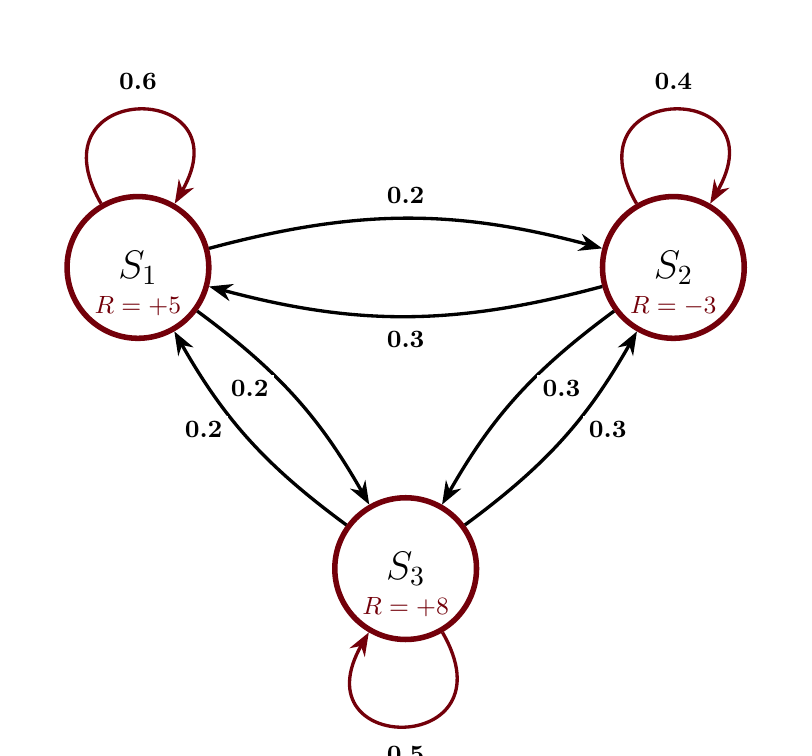
\begin{tikzpicture}[
    >=Stealth,
    scale=0.85,
    every state/.style={
        fill=white,
        draw=USC_Garnet,
        line width=2pt,
        text=black,
        minimum size=1.8cm,
        font=\bfseries\Large
    },
    every edge/.style={
        draw=black,
        line width=1.2pt,
        ->,
        >=Stealth
    },
    prob/.style={
        font=\bfseries\small,
        text=black,
        fill=white,
        inner sep=2pt
    },
    statelabel/.style={
        font=\small\bfseries,
        text=USC_Garnet
    }
]

% States
\node[state] (S1) at (0, 0) {$S_1$};
\node[statelabel, below=1pt of S1.center, yshift=-6pt] {$R=+5$};

\node[state] (S2) at (8, 0) {$S_2$};
\node[statelabel, below=1pt of S2.center, yshift=-6pt] {$R=-3$};

\node[state] (S3) at (4, -4.5) {$S_3$};
\node[statelabel, below=1pt of S3.center, yshift=-6pt] {$R=+8$};

% Self-loops
\path (S1) edge[loop above, looseness=5, out=120, in=60, draw=USC_Garnet] node[prob, above=5pt] {0.6} (S1);
\path (S2) edge[loop above, looseness=5, out=120, in=60, draw=USC_Garnet] node[prob, above=5pt] {0.4} (S2);
\path (S3) edge[loop below, looseness=5, out=-60, in=-120, draw=USC_Garnet] node[prob, below=5pt] {0.5} (S3);

% S1 <-> S2
\path (S1) edge[bend left=15] node[prob, above=3pt] {0.2} (S2);
\path (S2) edge[bend left=15] node[prob, below=3pt] {0.3} (S1);

% S1 <-> S3
\path (S1) edge[bend left=12] node[prob, left=4pt, pos=0.45] {0.2} (S3);
\path (S3) edge[bend left=12] node[prob, left=4pt, pos=0.55] {0.2} (S1);

% S2 <-> S3
\path (S2) edge[bend right=12] node[prob, right=4pt, pos=0.45] {0.3} (S3);
\path (S3) edge[bend right=12] node[prob, right=4pt, pos=0.55] {0.3} (S2);

\end{tikzpicture}
\end{center}

The transition matrix and reward vector are:
\[
\mathcal{P} = \begin{pmatrix}
0.6 & 0.2 & 0.2 \\
0.3 & 0.4 & 0.3 \\
0.2 & 0.3 & 0.5
\end{pmatrix}, \qquad
\mathbf{R} = \begin{pmatrix} +5 \\ -3 \\ +8 \end{pmatrix}
\]

\begin{enumerate}[label=(\alph*)]
\item Write the Bellman equation for this MRP in matrix form for a general discount factor $\gamma$. That is, express $\mathbf{V}$ as a function of $\mathbf{R}$, $\gamma$, and $\mathcal{P}$.

\vspace{4cm}

\item Form the matrix $(\mathbf{I} - \gamma \mathcal{P})$ explicitly for $\gamma = 0.8$. Show all entries.

\vspace{5cm}

\item Solve the $3 \times 3$ linear system $(\mathbf{I} - \gamma \mathcal{P})\mathbf{V} = \mathbf{R}$ for $\gamma = 0.8$ to find $V(S_1)$, $V(S_2)$, and $V(S_3)$. Show your work (Gaussian elimination, Cramer's rule, or equivalent).

\vspace{8cm}
\end{enumerate}

% ============================================================================
% PROBLEM 2: Discount Factor Analysis
% ============================================================================

\question{Problem 2: MRP Discount Factor Analysis}\label{prob:discount}

Use the same MRP from Problem~1.

\begin{enumerate}[label=(\alph*)]
\item Compute $V(S_1)$, $V(S_2)$, and $V(S_3)$ for $\gamma = 0$. Briefly explain why the answer is immediate.

\vspace{3cm}

\item Compute $V(S_1)$, $V(S_2)$, and $V(S_3)$ for $\gamma = 0.5$.

\vspace{7cm}

\item For approximately what value of $\gamma$ does $V(S_2)$ cross from negative to positive? Set $V(S_2) = 0$ in the Bellman equation and solve (you may approximate).

\vspace{5cm}

\item On the axes below, sketch the curves $V(S_1)$, $V(S_2)$, and $V(S_3)$ as functions of $\gamma \in [0, 1)$. Label each curve and mark the zero-crossing from part~(c).

\begin{center}
\begin{tikzpicture}
\begin{axis}[
    width=0.85\textwidth,
    height=7cm,
    xlabel={$\gamma$},
    ylabel={$V(s)$},
    xmin=0, xmax=1,
    ymin=-10, ymax=50,
    ymajorgrids=true,
    grid style={USC_Black10},
    axis lines=left,
    every axis x label/.style={at={(ticklabel* cs:1.0)}, anchor=west},
    every axis y label/.style={at={(ticklabel* cs:1.0)}, anchor=south},
    extra y ticks={0},
    extra y tick style={grid=major, grid style={black, line width=0.5pt}},
]
\end{axis}
\end{tikzpicture}
\end{center}
\end{enumerate}

% ============================================================================
% PROBLEM 3: Value Iteration by Hand
% ============================================================================

\question{Problem 3: Value Iteration by Hand}\label{prob:vi}

Consider the following MDP with states $\{X, Y\}$ and a terminal state $Z_T$, discount factor $\gamma = 0.9$. Each non-terminal state has two actions: $a_1$ and $a_2$. All transitions are deterministic.

\begin{center}
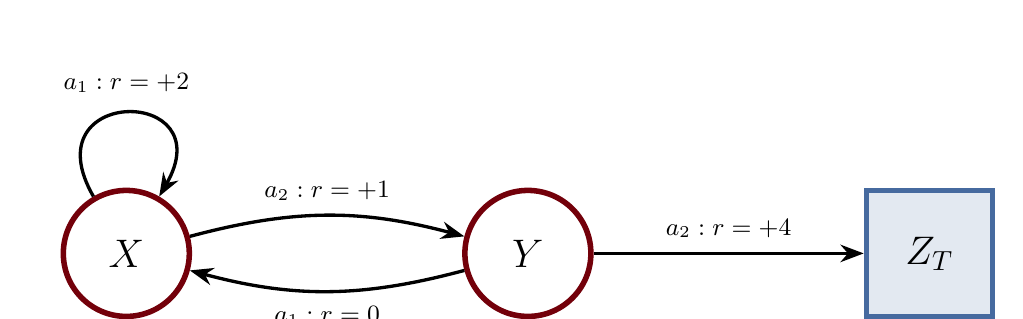
\begin{tikzpicture}[
    >=Stealth,
    scale=0.85,
    every state/.style={
        fill=white,
        draw=USC_Garnet,
        line width=2pt,
        text=black,
        minimum size=1.6cm,
        font=\bfseries\Large
    },
    every edge/.style={draw=black, line width=1.2pt, ->, >=Stealth},
    prob/.style={font=\small\bfseries, fill=white, inner sep=2pt},
    term/.style={
        fill=USC_Atlantic!15,
        draw=USC_Atlantic,
        line width=2pt,
        text=black,
        minimum size=1.6cm,
        font=\bfseries\Large
    }
]

\node[state] (X) at (0, 0) {$X$};
\node[state] (Y) at (6, 0) {$Y$};
\node[term] (Z) at (12, 0) {$Z_T$};

% X actions
\path (X) edge[loop above, looseness=5, out=120, in=60] node[prob, above=5pt] {$a_1: r=+2$} (X);
\path (X) edge[bend left=15] node[prob, above=3pt] {$a_2: r=+1$} (Y);

% Y actions
\path (Y) edge[bend left=15] node[prob, below=3pt] {$a_1: r=0$} (X);
\path (Y) edge node[prob, above=3pt] {$a_2: r=+4$} (Z);

\end{tikzpicture}
\end{center}

\textbf{Transition and reward summary:}
\begin{center}
\begin{tabular}{cccc}
\toprule
\textbf{State} & \textbf{Action} & \textbf{Next State} & \textbf{Reward} \\
\midrule
$X$ & $a_1$ & $X$ & $+2$ \\
$X$ & $a_2$ & $Y$ & $+1$ \\
$Y$ & $a_1$ & $X$ & $0$ \\
$Y$ & $a_2$ & $Z_T$ & $+4$ \\
\bottomrule
\end{tabular}
\end{center}

\begin{enumerate}[label=(\alph*)]
\item Initialize $V_0(X) = V_0(Y) = 0$. Perform \textbf{3 iterations} of value iteration. Fill in the table below. Show computation for each cell.

\begin{center}
\begin{tabular}{ccccc}
\toprule
\textbf{Iter $k$} & $V_k(X)$ & $\pi_k(X)$ & $V_k(Y)$ & $\pi_k(Y)$ \\
\midrule
0 & 0 & --- & 0 & --- \\[0.5em]
1 & & & & \\[0.5em]
2 & & & & \\[0.5em]
3 & & & & \\
\bottomrule
\end{tabular}
\end{center}

\vspace{6cm}

\item After convergence, what is the optimal policy $\pi^*$? State $\pi^*(X)$ and $\pi^*(Y)$ and justify briefly.

\vspace{3cm}

\item Compute the exact optimal values $V^*(X)$ and $V^*(Y)$ by solving the Bellman optimality equations simultaneously (not by iteration).

\vspace{5cm}
\end{enumerate}

% ============================================================================
% PROBLEM 4: Grid World Policy
% ============================================================================

\question{Problem 4: Grid World Policy}\label{prob:grid}

Consider the $3 \times 3$ grid MDP below. The agent can move \textbf{Up, Down, Left, Right}. Moves that would leave the grid keep the agent in place. All transitions are deterministic. Discount factor $\gamma = 1$.

\begin{center}
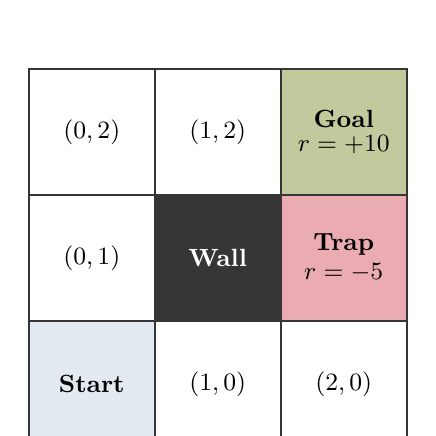
\begin{tikzpicture}[
    cell/.style={minimum size=1.6cm, draw=USC_Black90, line width=0.8pt, font=\small, anchor=center}
]

% Row 2 (top)
\node[cell, fill=white] at (0, 3.2) {$(0,2)$};
\node[cell, fill=white] at (1.6, 3.2) {$(1,2)$};
\node[cell, fill=USC_Horseshoe!40, font=\small\bfseries] at (3.2, 3.2) {\shortstack{Goal\\$r=+10$}};

% Row 1 (middle)
\node[cell, fill=white] at (0, 1.6) {$(0,1)$};
\node[cell, fill=USC_Black90, text=white, font=\small\bfseries] at (1.6, 1.6) {Wall};
\node[cell, fill=USC_Rose!40, font=\small\bfseries] at (3.2, 1.6) {\shortstack{Trap\\$r=-5$}};

% Row 0 (bottom)
\node[cell, fill=USC_Atlantic!15, font=\small\bfseries] at (0, 0) {Start};
\node[cell, fill=white] at (1.6, 0) {$(1,0)$};
\node[cell, fill=white] at (3.2, 0) {$(2,0)$};

\end{tikzpicture}
\end{center}

\textbf{Rules:}
\begin{itemize}[nosep]
\item Every move costs $r = -1$ (step penalty), except moves into Goal or Trap.
\item Reaching the \textbf{Goal} $(2,2)$: reward $r = +10$, episode ends.
\item Reaching the \textbf{Trap} $(2,1)$: reward $r = -5$, episode ends.
\item The \textbf{Wall} $(1,1)$ is impassable; moves into it keep the agent in place (still costs $-1$).
\item Goal and Trap are terminal states.
\end{itemize}

\begin{enumerate}[label=(\alph*)]
\item List the reward $R(s, a, s')$ for every non-terminal state $s$ and every action $a$. Organize your answer clearly (a table is fine).

\vspace{6cm}

\item Starting from $V_0(s) = 0$ for all states, perform \textbf{2 iterations} of value iteration. Write the resulting values in each cell of the grids below.

\textbf{After Iteration 1:}
\begin{center}
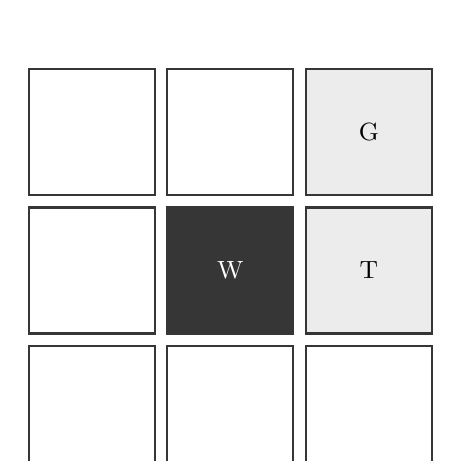
\begin{tikzpicture}[
    scale=1.1,
    cell/.style={minimum size=1.6cm, draw=USC_Black90, line width=0.8pt, font=\small, anchor=center}
]
\node[cell] at (0, 3.2) {};
\node[cell] at (1.6, 3.2) {};
\node[cell, fill=USC_Black10] at (3.2, 3.2) {G};
\node[cell] at (0, 1.6) {};
\node[cell, fill=USC_Black90, text=white] at (1.6, 1.6) {W};
\node[cell, fill=USC_Black10] at (3.2, 1.6) {T};
\node[cell] at (0, 0) {};
\node[cell] at (1.6, 0) {};
\node[cell] at (3.2, 0) {};
\end{tikzpicture}
\end{center}

\textbf{After Iteration 2:}
\begin{center}
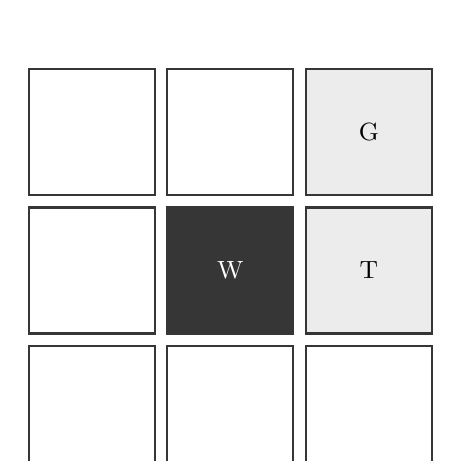
\begin{tikzpicture}[
    scale=1.1,
    cell/.style={minimum size=1.6cm, draw=USC_Black90, line width=0.8pt, font=\small, anchor=center}
]
\node[cell] at (0, 3.2) {};
\node[cell] at (1.6, 3.2) {};
\node[cell, fill=USC_Black10] at (3.2, 3.2) {G};
\node[cell] at (0, 1.6) {};
\node[cell, fill=USC_Black90, text=white] at (1.6, 1.6) {W};
\node[cell, fill=USC_Black10] at (3.2, 1.6) {T};
\node[cell] at (0, 0) {};
\node[cell] at (1.6, 0) {};
\node[cell] at (3.2, 0) {};
\end{tikzpicture}
\end{center}

\vspace{4cm}

\item On the grid below, draw the optimal policy (one arrow per non-terminal cell indicating the best action).

\begin{center}
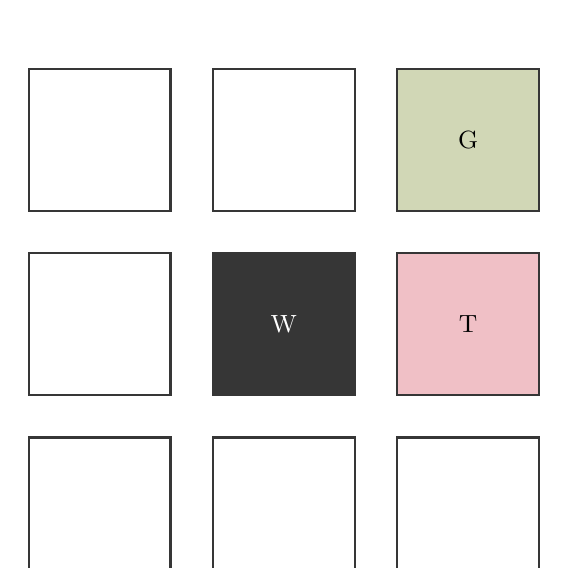
\begin{tikzpicture}[
    scale=1.3,
    cell/.style={minimum size=1.8cm, draw=USC_Black90, line width=0.8pt, font=\small, anchor=center}
]
\node[cell] at (0, 3.6) {};
\node[cell] at (1.8, 3.6) {};
\node[cell, fill=USC_Horseshoe!30] at (3.6, 3.6) {G};
\node[cell] at (0, 1.8) {};
\node[cell, fill=USC_Black90, text=white] at (1.8, 1.8) {W};
\node[cell, fill=USC_Rose!30] at (3.6, 1.8) {T};
\node[cell] at (0, 0) {};
\node[cell] at (1.8, 0) {};
\node[cell] at (3.6, 0) {};
\end{tikzpicture}
\end{center}
\end{enumerate}

% ============================================================================
% PROBLEM 5: Q-Learning Episode Trace
% ============================================================================

\question{Problem 5: Q-Learning Episode Trace}\label{prob:qlearn}

Consider the following 2-state MDP with states $\{A, B\}$ and terminal state $B_T$. Each state has two actions: $L$ and $R$.

\begin{center}
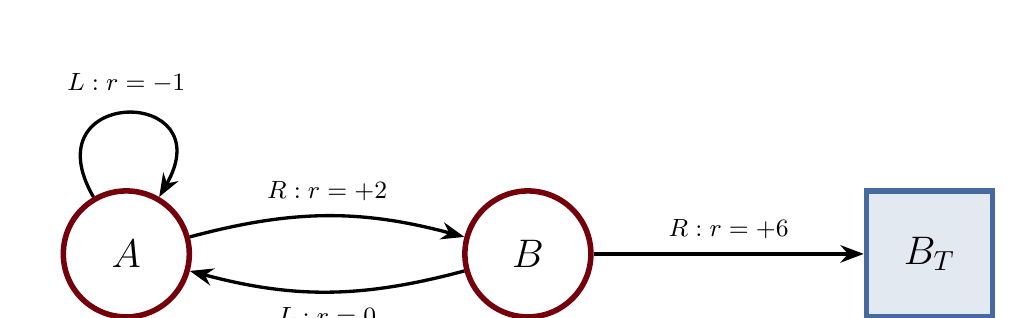
\begin{tikzpicture}[
    >=Stealth,
    scale=0.85,
    every state/.style={
        fill=white,
        draw=USC_Garnet,
        line width=2pt,
        text=black,
        minimum size=1.6cm,
        font=\bfseries\Large
    },
    every edge/.style={draw=black, line width=1.2pt, ->, >=Stealth},
    prob/.style={font=\small\bfseries, fill=white, inner sep=2pt},
    term/.style={
        fill=USC_Atlantic!15,
        draw=USC_Atlantic,
        line width=2pt,
        text=black,
        minimum size=1.6cm,
        font=\bfseries\Large
    }
]

\node[state] (A) at (0, 0) {$A$};
\node[state] (B) at (6, 0) {$B$};
\node[term] (BT) at (12, 0) {$B_T$};

% A actions
\path (A) edge[loop above, looseness=5, out=120, in=60] node[prob, above=5pt] {$L: r=-1$} (A);
\path (A) edge[bend left=15] node[prob, above=3pt] {$R: r=+2$} (B);

% B actions
\path (B) edge[bend left=15] node[prob, below=3pt] {$L: r=0$} (A);
\path (B) edge node[prob, above=3pt] {$R: r=+6$} (BT);

\end{tikzpicture}
\end{center}

All transitions are deterministic. Use \textbf{Q-learning} with $\alpha = 0.2$, $\gamma = 1$, and $\varepsilon = 0$ (pure greedy; break ties alphabetically by action name, i.e., $L$ before $R$).

Initialize all Q-values to zero: $Q(A,L) = Q(A,R) = Q(B,L) = Q(B,R) = 0$.

The three episode trajectories are given (not chosen by your policy---just apply the updates):

\textbf{Episode 1:} $A \xrightarrow{R} B \xrightarrow{R} B_T$

\textbf{Episode 2:} $A \xrightarrow{R} B \xrightarrow{R} B_T$

\textbf{Episode 3:} $A \xrightarrow{L} A \xrightarrow{R} B \xrightarrow{R} B_T$

\begin{enumerate}[label=(\alph*)]
\item For each step of each episode, compute the Q-learning update. Fill in the table.

\textit{Recall:} $Q(s,a) \leftarrow Q(s,a) + \alpha\big[r + \gamma \max_{a'} Q(s',a') - Q(s,a)\big]$

\begin{center}
\begin{tabular}{ccccccl}
\toprule
\textbf{Ep.} & \textbf{Step} & $\mathbf{s}$ & $\mathbf{a}$ & $\mathbf{s'}$ & $\mathbf{r}$ & \textbf{New $Q(s,a)$} \\
\midrule
1 & 1 & $A$ & $R$ & $B$ & $+2$ & \\[0.4em]
1 & 2 & $B$ & $R$ & $B_T$ & $+6$ & \\[0.4em]
\midrule
2 & 1 & $A$ & $R$ & $B$ & $+2$ & \\[0.4em]
2 & 2 & $B$ & $R$ & $B_T$ & $+6$ & \\[0.4em]
\midrule
3 & 1 & $A$ & $L$ & $A$ & $-1$ & \\[0.4em]
3 & 2 & $A$ & $R$ & $B$ & $+2$ & \\[0.4em]
3 & 3 & $B$ & $R$ & $B_T$ & $+6$ & \\[0.4em]
\bottomrule
\end{tabular}
\end{center}

\vspace{5cm}

\item State all four Q-values after the 3 episodes are complete.

\vspace{3cm}

\item What is the greedy policy $\pi(s) = \arg\max_a Q(s,a)$ for each state?

\vspace{2cm}
\end{enumerate}

% ============================================================================
% PROBLEM 6: Exploration vs Exploitation
% ============================================================================

\question{Problem 6: Exploration vs.\ Exploitation}\label{prob:explore}

\begin{enumerate}[label=(\alph*)]
\item Suppose an agent is in a state with three available actions $\{a_1, a_2, a_3\}$ and current Q-values:
\[
Q(s, a_1) = 5.0, \qquad Q(s, a_2) = 3.2, \qquad Q(s, a_3) = 7.1
\]
Under an $\varepsilon$-greedy policy with $\varepsilon = 0.4$, compute the probability of selecting each action. Show your work.

\vspace{5cm}

\item Suppose $\varepsilon$ starts at $\varepsilon_0 = 1.0$ and decays multiplicatively each episode by a factor of $0.99$:
\[
\varepsilon_k = \varepsilon_0 \cdot 0.99^k
\]
After how many episodes $k$ is $\varepsilon_k < 0.05$? Solve exactly using logarithms.

\vspace{5cm}

\item In 3--5 sentences, explain: Why is exploration important in the early stages of learning? Why is it beneficial to decay $\varepsilon$ over time rather than keeping it fixed?

\vspace{5cm}
\end{enumerate}

% ============================================================================
% END OF DOCUMENT
% ============================================================================

\end{document}
